\chapter{Hardware and Software}\label{cha:hardware}
This chapter describes the hardware used in the thesis. The \abbrROV frame and thrusters was a package from BlueRobotics. In addition to the \abbrROV frame, a Raspberry pi was used as an onboard computer and a HKPilot Mega 2.7  was used as a input/output (\abbrIO) unit. The software in the \abbrROV was built on top of \abbrROS. In \Appref{app:dependencies} and \Appref{app:operation} instruction for installation of software and instructions for using the \abbrROV can be found.

\section{BlueROV Package}
In this thesis the BlueRov from BlueRobotics was used. The BlueROV package, see \Figureref{fig:bluerov}, includes the acrylic chassi, acrylic tube, six electronic speed controllers, six BlueRobotics T200 thrusters, cable penetrators and a cradle for mounting of electronics.
\missingfigure{Missing figure of the bluerov package}
\section{\abbrROV \abbrIO}
The \abbrROV's \abbrIO consists of an HKPilot Mega 2.7 which is based on Ardupilot Mega. The HKPilot Mega 2.7 has the following on chip sensors
\begin{itemize}
    \item Magnetometer - HMC5883L.
    \item Barometer - MS5611-01BA.
    \item Inertial measurement unit (\abbrIMU) - MPU6000.
\end{itemize}
An external pressure sensor MS5837-30BA which was encased in a watertight case by BlueRobotics was connected to the HKPilot Mega 2.7 by \abbrIC.
The HKPilot Mega 2.7 also controls the six \abbrESC. The \abbrESC's are 30A AfroESC's flashed with BlueRobotics linearising software. The HKPilot Mega 2.7 is connected to the onboard computer by \abbrUSB cable.The HKPilot Mega 2.7 runs a rosserial-arduino node which is a lite \abbrROS node that communicates with a master node by serial communication. Scaling calibration of the sensors are done automatically. However, the offset of the magnetometer and \abbrROV has to be done manually by following the instructions that are produced in the workstation terminal window. The external pressure sensor uses the internal barometer to remove the atmospheric pressure offset. The atmospheric pressure offset is measured at the start up of the \abbrROV.

\section{Power}
To power the \abbrROV a Turnigy 5000mAh 4S 25C Lipo Pack was used. This is a high discharge battery which ensures that all thrusters can be run at the same time without any voltage drops.
To power the Raspberry pi 2 a HobbyKing LIPO to USB Charging Adapter was used. This adapter connects to the JST-XH connector on the Lipo battery and then outputs regular USB voltages and currents. A \abbrUSB to micro-\abbrUSB adapter was used to route the power to the Raspberry pi. 
The speed controllers are powered via the main lead of the Lipo battery. Lastly the HKPilot Mega 2.7 is powered by the Raspberry and by the speed controllers. 

\section{Onboard Computer}
The onboard computer was a Raspberry pi 2 Model B which can be seen in \Figureref{fig:raspberryandcamera}. To the Raspberry pi 2 a Raspicam is connected. 
Nodes running on the onboard computer can be seen in \Tableref{tab:raspnodes}.
 \begin{table}[tbp]
  \centering
  \caption{\label{tab:raspnodes}%
    The different nodes that run on the onboard computer.}

  \begin{tabular}{l p{0.5\linewidth}}
    \toprule%
    \textbf{Node} & \textbf{Description} \\
    \otoprule%
    roscore             &  Node that handles the \abbrROS backend.\\

    raspicam\_node      &  Camera node for streaming video from the \abbrROV.\\
    
    controller          &  Simulink generated node that can run different controllers.\\
    
    rosserial           &  Serial node for communication with the HKPilot Mega 2.7.\\
    
    matlab\_controller  &  Dynamic reconfigure node for the controller node.\\
    \bottomrule%
  \end{tabular}
\end{table}

\begin{figure}
    \centering
    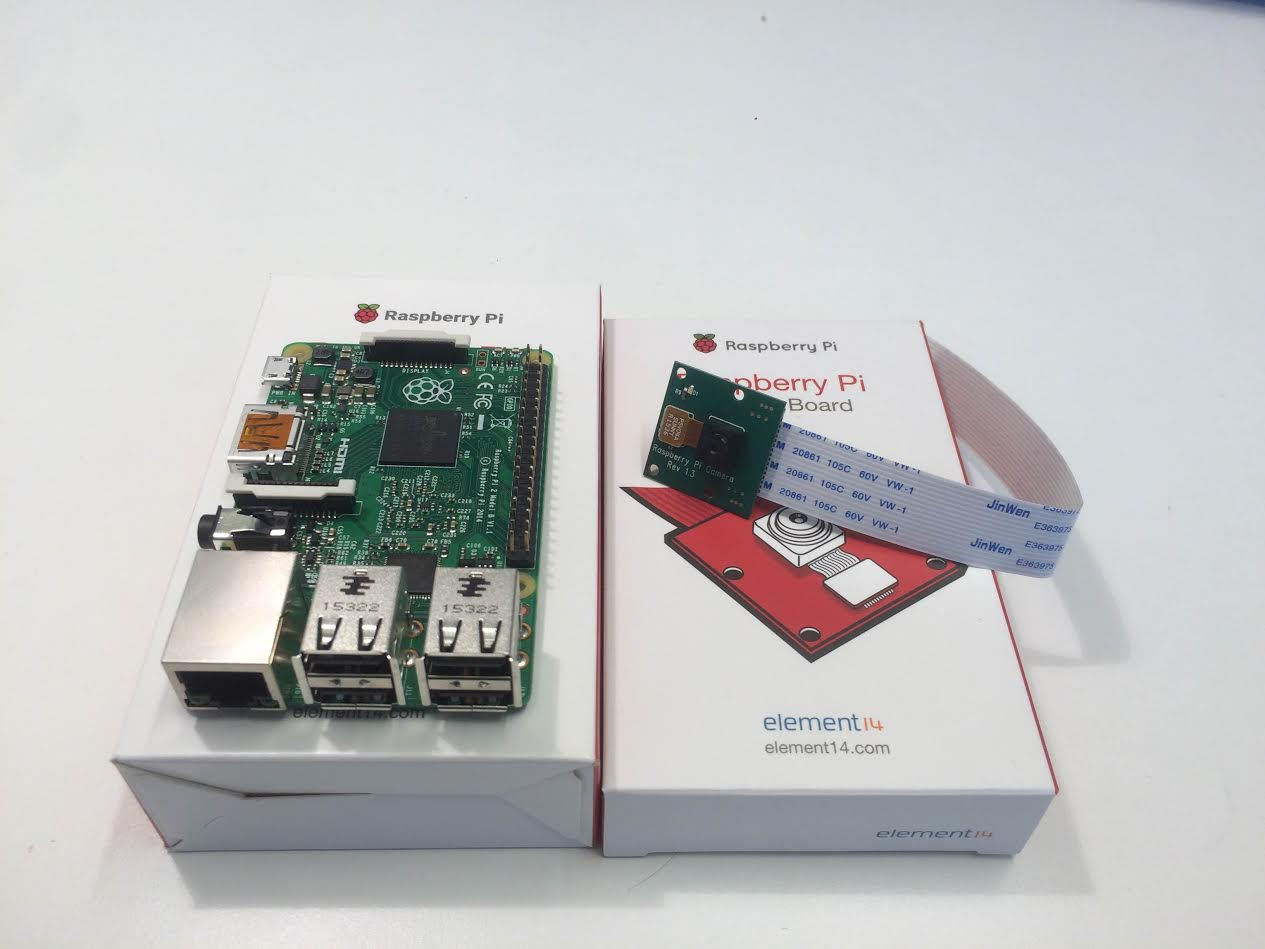
\includegraphics[trim={0 0 0 5cm},clip,width=0.9\textwidth]{raspberryandcamera}
    \caption{The Raspberry pi 2 Model B, the onboard computer, is shown to the left and the raspicam is shown on the right.}
    \label{fig:raspberryandcamera}
\end{figure}

\section{Workstation}
The used workstation computer in the thesis is a Lenovo T430 with i5-3210M processor and Intel\textregistered HD Graphics 4000. The workstation was connected via a tether to the Raspberry pi 2 which in our case was a cat 6 cable.
\begin{table}[tbp]
  \centering
  \caption{\label{tab:workstationnodes}%
    The different node that run on the workstation.}

  \begin{tabular}{l p{0.5\linewidth}}
    \toprule%
    \textbf{Node} & \textbf{Description} \\
    \otoprule%
    heartbeat       & Node for checking the connection with the HKPilot Mega 2.7.\\

    teleop\_xbox    & Xbox node for handling inputs from the xbox controller.\\

    joy             & A joystick node for interacting with the \abbrOS:s \abbrUSB inputs.\\
        
    
    rqt             & A \abbrGUI for the \abbrROV.\\
    
    sensorfusion    & The sensor fusion node. \\
    \bottomrule%
  \end{tabular}
\end{table}